\begin{figure}[t]
	\centering
	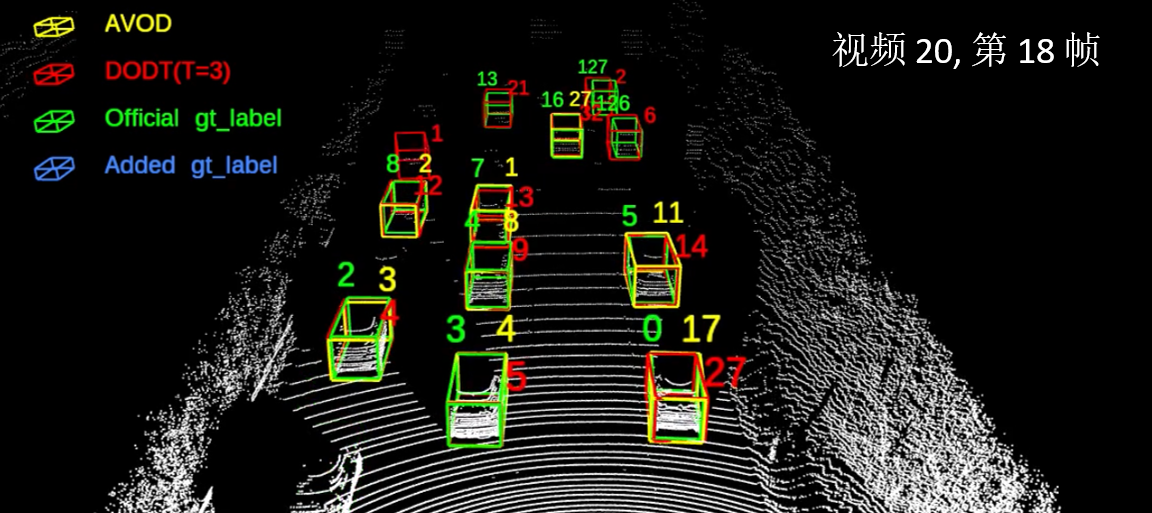
\includegraphics[width=\textwidth]{./imgs/viz_results/val/avod_dodt_01.png}\vspace{1pt}
	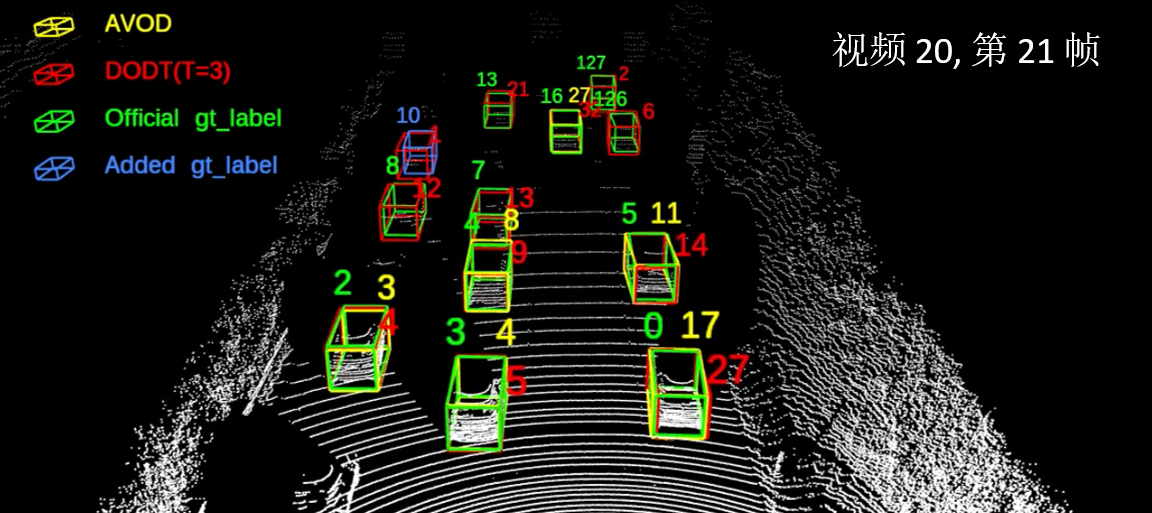
\includegraphics[width=\textwidth]{./imgs/viz_results/val/avod_dodt_02.png}\vspace{1pt}
	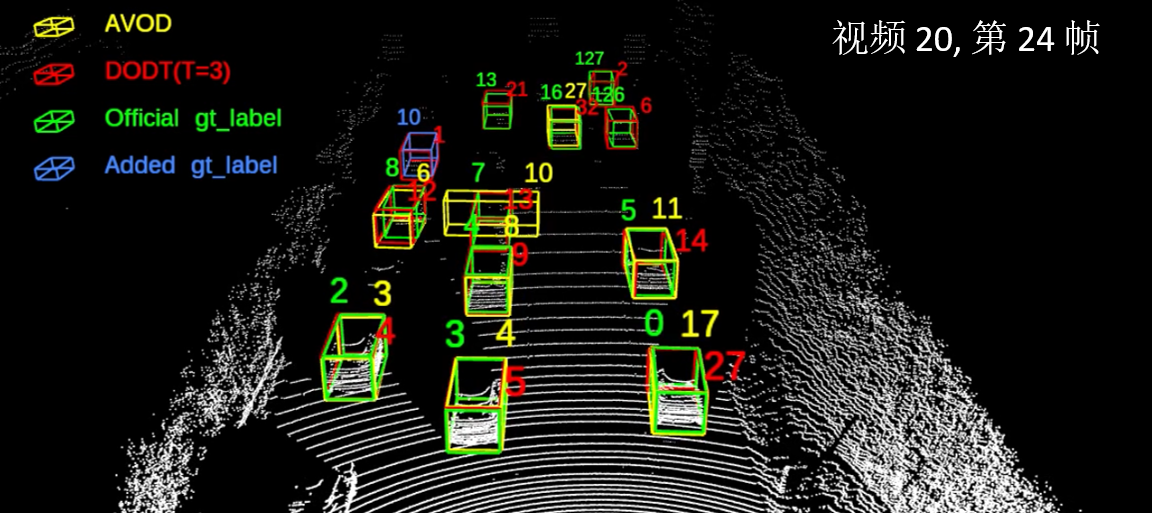
\includegraphics[width=\textwidth]{./imgs/viz_results/val/avod_dodt_03.png}
	\caption{AVOD与DODT($\tau=3$)对比结果,可以看出相比于AVOD,DODT(T=3) 对远处目标以及新添加标签的目标预测更好。}
	\label{fig:avod_dodt}
\end{figure}

\begin{figure}[t]
	\centering
	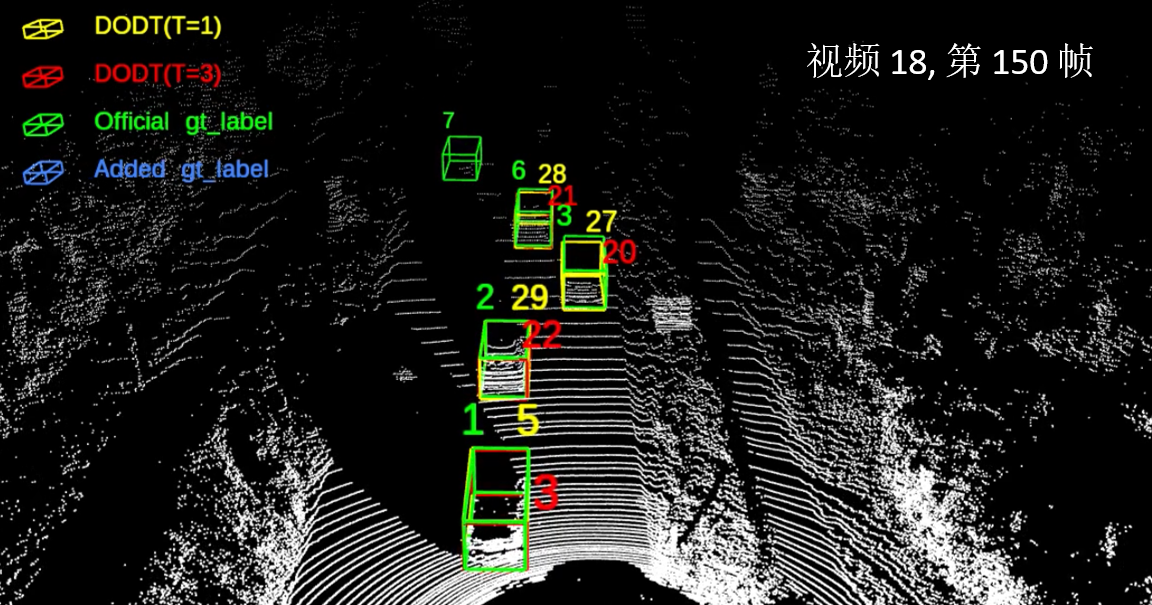
\includegraphics[width=\textwidth]{./imgs/viz_results/val/dodt_1_3_01.png}\vspace{1pt}
	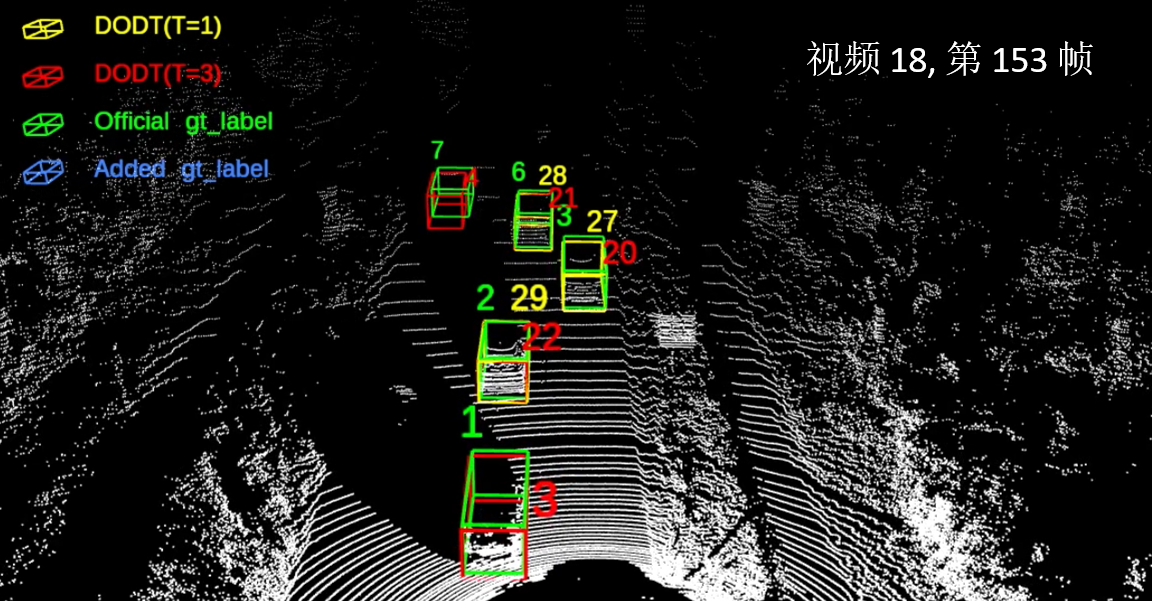
\includegraphics[width=\textwidth]{./imgs/viz_results/val/dodt_1_3_02.png}\vspace{1pt}
	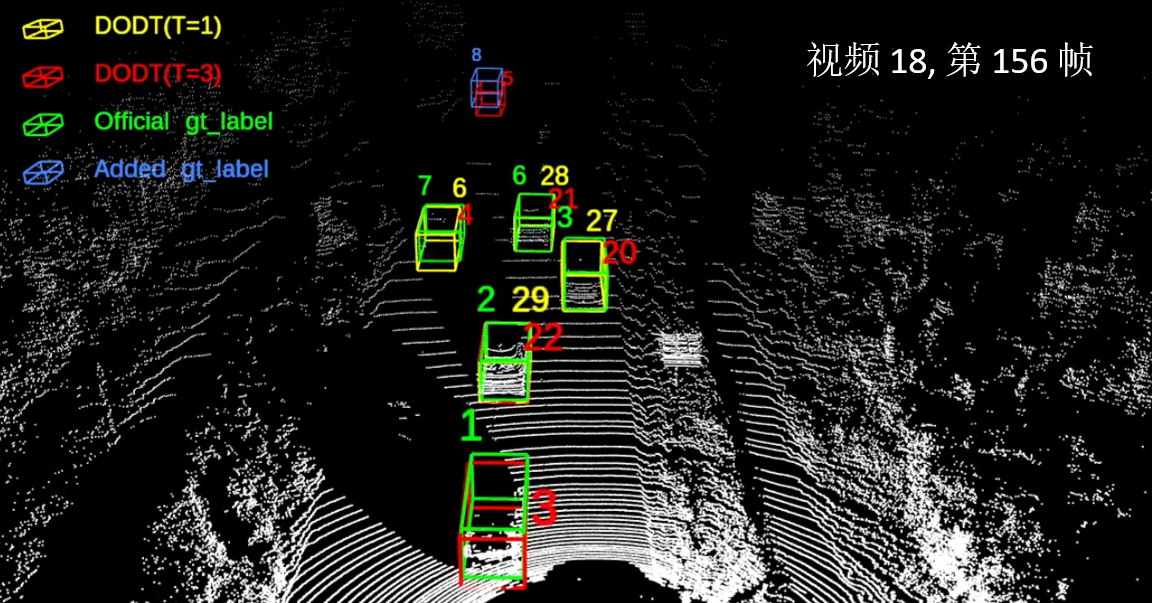
\includegraphics[width=\textwidth]{./imgs/viz_results/val/dodt_1_3_03.png}
	\caption{DODT($\tau=1$)与DODT($\tau=3$)对比结果,可以看出大步长有利于轨迹的延伸,从而使得模型对远处物体预测性能更好。}
	\label{fig:dodt_1_3}
\end{figure}

\begin{figure}[t]
	\centering
	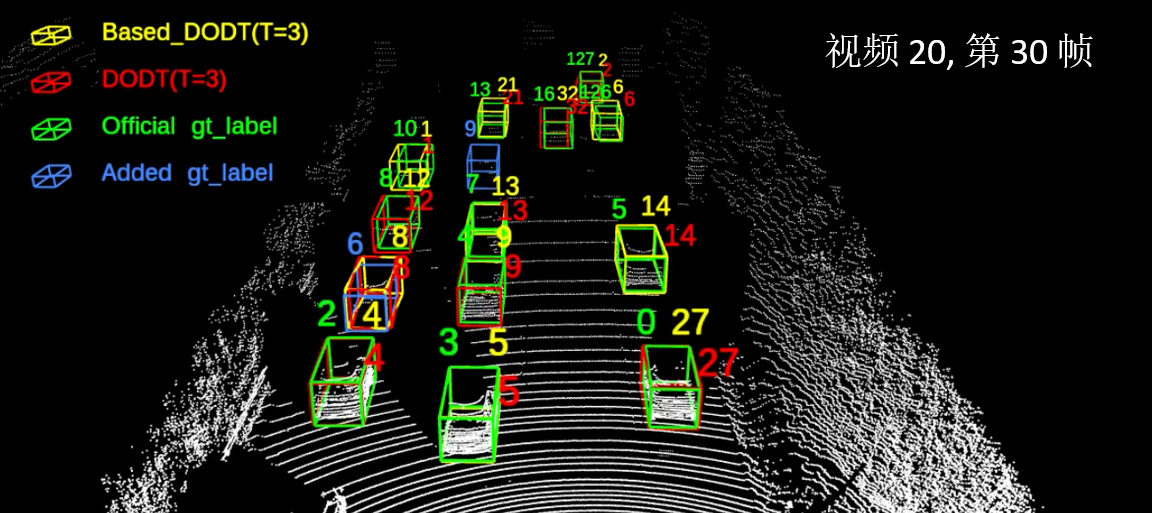
\includegraphics[width=\textwidth]{./imgs/viz_results/val/dodt_based_01.png}\vspace{1pt}
	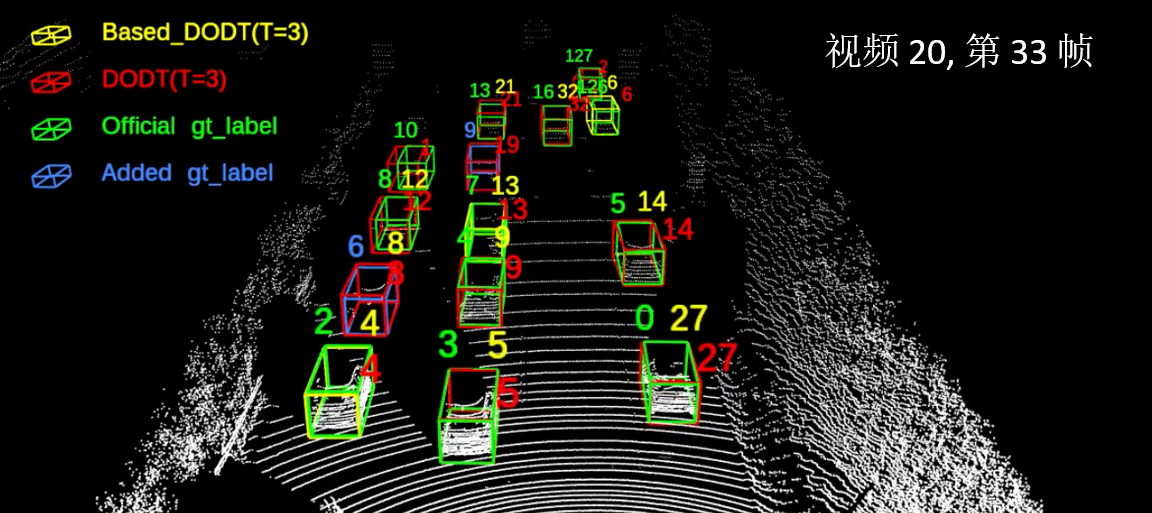
\includegraphics[width=\textwidth]{./imgs/viz_results/val/dodt_based_02.png}\vspace{1pt}
	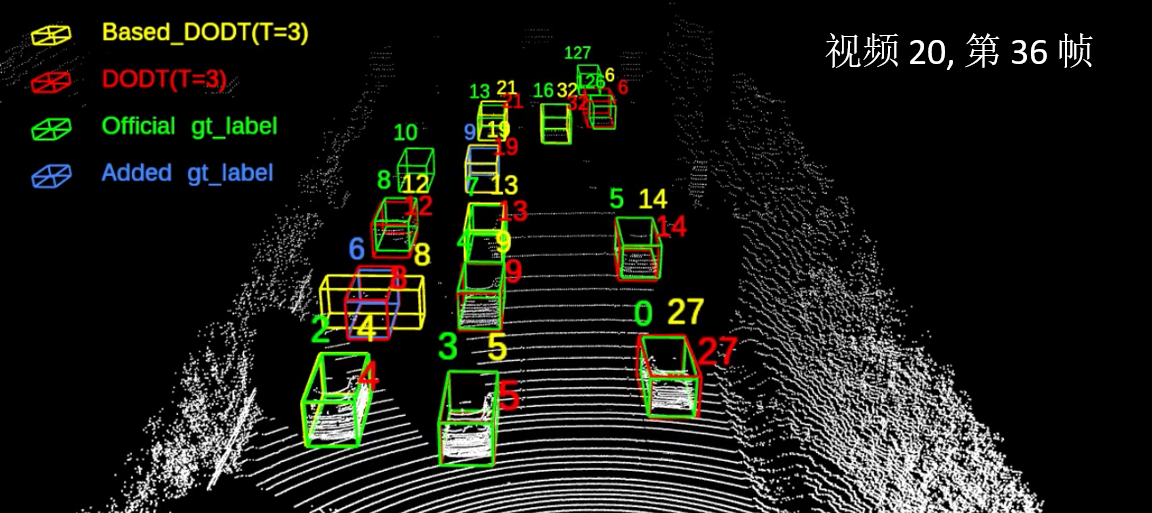
\includegraphics[width=\textwidth]{./imgs/viz_results/val/dodt_based_03.png}
	\caption{Based\_DODT与DODT($\tau=3$)对比结果,可以看出时序信息以及MoI插值算法有利于保持目标状态的长程连续性。}
	\label{fig:dodt_based}
\end{figure}
